\documentclass[12pt,a4paper]{article}
\usepackage[utf8]{inputenc}
\usepackage{amsmath}
\usepackage{amsfonts}
\usepackage{amssymb}
\usepackage{makeidx}
\usepackage{graphicx}
\usepackage{lmodern}
\usepackage{color}
\usepackage{xcolor}
\usepackage{bussproofs}
\usepackage{lscape}
\usepackage{listings}
\usepackage{amsthm}
\usepackage[left=2cm,right=2cm,top=2cm,bottom=2cm]{geometry}

\author{Mudathir Mahgoub}
\title{Symbolic Execution Engine}


\newtheorem*{remark}{\textbf{Remark}}

\begin{document}

\maketitle

\section {Project Problem}

\section{Software description} \label{sec:software}


\begin{figure}[h]
 \centering
 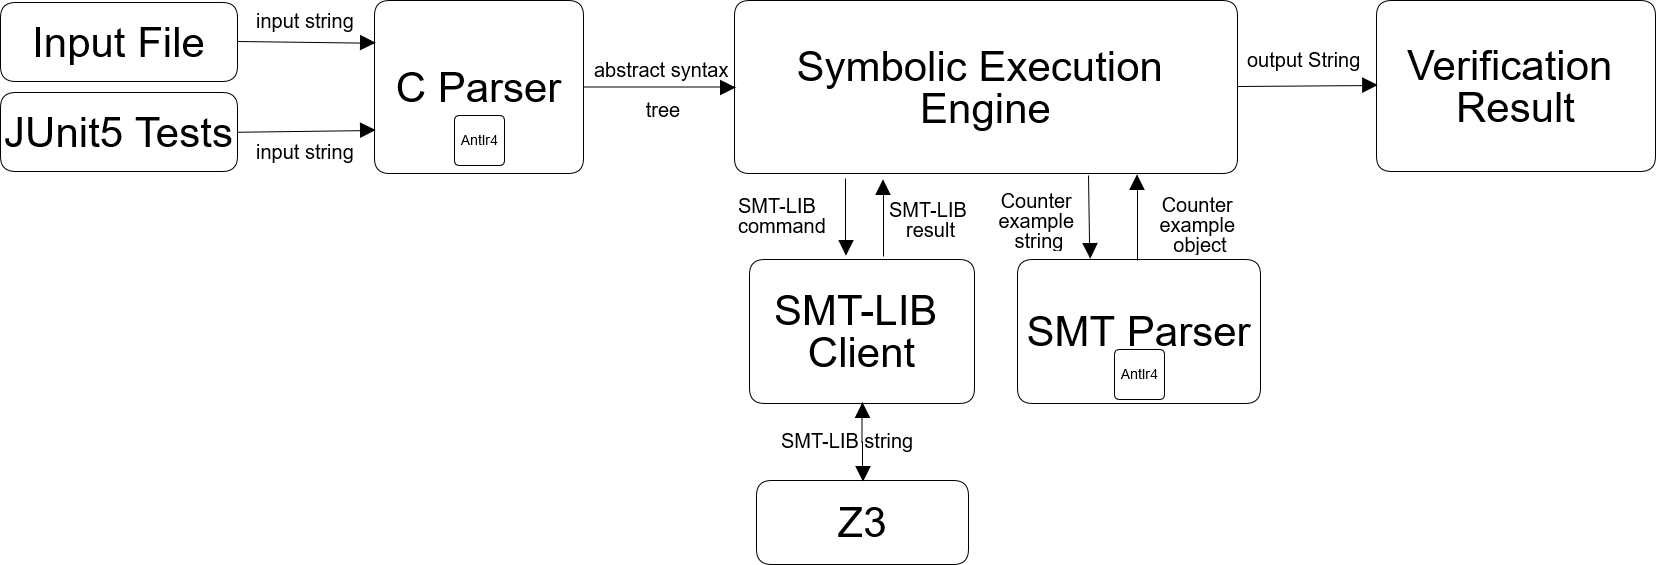
\includegraphics[scale=.25,keepaspectratio=true]{./engine.png}
 % gantt_chart.png: 0x0 pixel, 0dpi, nanxnan cm, bb=
 \caption{Project architecture.}
 \label{fig:gantt_chart}
\end{figure}

The project is implemented using Java and the executable is a jar file (target/TypeChecker.jar) which is generated using the command:
\definecolor{light-gray}{gray}{0.95}
\lstset{backgroundcolor= \color{light-gray}}

\begin{lstlisting}  
mvn install
\end{lstlisting}  

The program receives as an input a text file containing subtypes definitions and a judgment to be checked. For testing, \textbf{JUnit5} was used to test the program directly without files. The input is passed to the \textbf{Parser} which uses the ANTLR library to parse the input into an abstract syntax tree. This abstract syntax tree is consumed by the \textbf{Type Checker} which uses the rules in sections \ref{sec:simple} and \ref{sec:systemF} to build a derivation tree and determine the answer of the type checking. The answer can be \textbf{Yes}, \textbf{No}, or \textbf{Unknown}. Finally the derivation tree can be printed using the \textbf{Default Printer} or the \textbf{Latex Printer}.


Here is an example of an input:

\definecolor{light-gray}{gray}{0.95}

\lstset{caption={test.txt},backgroundcolor= \color{light-gray}}

\begin{lstlisting}  
SubBase(bool, int);
. |- \lambda x. \lambda y. (x y)[bool]: (int ->T) -> (bool -> T);
\end{lstlisting}

Here is the output of the default printer:

\lstset{caption={java -jar TypeChecker.jar -i test.txt}}

\begin{lstlisting}  
Yes
                                SubBase(bool, int)
-------------------(var)        -------------------(subBase)
x: bool ? x : bool                      bool <: int
--------------------------------------(subsumption)
x: bool ? x : int

\end{lstlisting}

Here is the output of the latex printer which uses bussproofs package centered proofs:

\lstset{caption={java -jar TypeChecker.jar -i test.txt -latex}}

\begin{lstlisting} 
Yes
\begin{prooftree}
\AxiomC{} \RightLabel{\scriptsize var}
\UnaryInfC{$x: bool \vdash x : bool$}
\AxiomC{\scriptsize $SubBase(bool,int)$}
\RightLabel{\scriptsize subBase}
\UnaryInfC{$bool <: int$}
\RightLabel{\scriptsize subsumption}
\BinaryInfC{$x: bool \vdash x : int$}
\end{prooftree}

\end{lstlisting} 

The following sections focus on terms and rules used in the \textbf{Type Checker}. 

\section{Simple types} \label{sec:simple}

\end{document}
